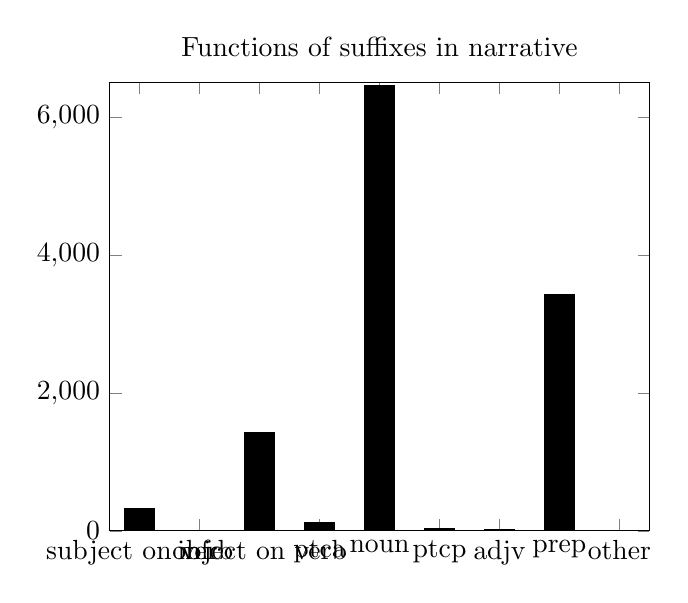
\begin{tikzpicture}[baseline]
\begin{axis}[
title = Functions of suffixes in narrative,
xmin=-0.5, xmax=8.5,
ymin=0, ymax=6500,
xtick={0,1,2,3,4,5,6,7,8},
xticklabels={subject on verb,infc,object on verb,ptca,noun,ptcp,adjv,prep,other},
xticklabel style = {\xticklabel},
]
\draw[draw=\bardrawcolor,fill=\barcolor] (axis cs:-0.25,0) rectangle (axis cs:0.25,323);
\draw[draw=\bardrawcolor,fill=\barcolor] (axis cs:0.75,0) rectangle (axis cs:1.25,3);
\draw[draw=\bardrawcolor,fill=\barcolor] (axis cs:1.75,0) rectangle (axis cs:2.25,1427);
\draw[draw=\bardrawcolor,fill=\barcolor] (axis cs:2.75,0) rectangle (axis cs:3.25,123);
\draw[draw=\bardrawcolor,fill=\barcolor] (axis cs:3.75,0) rectangle (axis cs:4.25,6458);
\draw[draw=\bardrawcolor,fill=\barcolor] (axis cs:4.75,0) rectangle (axis cs:5.25,39);
\draw[draw=\bardrawcolor,fill=\barcolor] (axis cs:5.75,0) rectangle (axis cs:6.25,20);
\draw[draw=\bardrawcolor,fill=\barcolor] (axis cs:6.75,0) rectangle (axis cs:7.25,3431);
\draw[draw=\bardrawcolor,fill=\barcolor] (axis cs:7.75,0) rectangle (axis cs:8.25,1);
\end{axis}
\end{tikzpicture}

